\documentclass[11pt]{article}


\usepackage{fullpage}
\usepackage{graphicx}
\usepackage{amsmath}
\usepackage{amssymb}
\usepackage{amsthm}
\usepackage{fancyvrb}

\newcommand{\myname}{Mehshan Mustafa}

\newenvironment{theorem}[2][Theorem]{\begin{trivlist}
\item[\hskip \labelsep {\bfseries #1}\hskip \labelsep {\bfseries #2.}]}{\end{trivlist}}
\newenvironment{lemma}[2][Lemma]{\begin{trivlist}
\item[\hskip \labelsep {\bfseries #1}\hskip \labelsep {\bfseries #2.}]}{\end{trivlist}}
\newenvironment{exercise}[2][Exercise]{\begin{trivlist}
\item[\hskip \labelsep {\bfseries #1}\hskip \labelsep {\bfseries #2.}]}{\end{trivlist}}
\newenvironment{problem}[2][Problem]{\begin{trivlist}
\item[\hskip \labelsep {\bfseries #1}\hskip \labelsep {\bfseries #2.}]}{\end{trivlist}}
\newenvironment{question}[2][Question]{\begin{trivlist}
\item[\hskip \labelsep {\bfseries #1}\hskip \labelsep {\bfseries #2.}]}{\end{trivlist}}
\newenvironment{corollary}[2][Corollary]{\begin{trivlist}
\item[\hskip \labelsep {\bfseries #1}\hskip \labelsep {\bfseries #2.}]}{\end{trivlist}}
\newenvironment{solution}{\begin{proof}[Solution]}{\end{proof}}
\newenvironment{idea}[2][Proof Idea.]{\textit{#1} #2}



\parindent0in
\pagestyle{plain}
\thispagestyle{plain}

\usepackage{csquotes}
\usepackage[shortlabels]{enumitem}

\newcommand{\dated}{\today}
\newcommand{\token}[1]{\langle \text{#1} \rangle}

\begin{document}

\textbf{Introduction to the Theory of
Computation}\hfill\textbf{\myname}\\[0.01in]
\textbf{Chapter 7: Time Complexity}\hfill\textbf{\dated}\\
\smallskip\hrule\bigskip

\begin{problem}{7.28}
You are given a box and a collection of cards as indicated in the following figure.
Because of the pegs in the box and the notches in the cards, each card will fit in the
box in either of two ways. Each card contains two columns of holes, some of which
may not be punched out. The puzzle is solved by placing all the cards in the box
so as to completely cover the bottom of the box (i.e., every hole position is blocked
by at least one card that has no hole there). Let $PUZZLE = \{\langle c_1, \cdots, c_k \rangle \ | \text{ each } c_i \text{ represents a card and this collection of cards has a solution}\}$. Show that $PUZZLE$ is NP-complete.
\end{problem}

\begin{proof}
To show that $PUZZLE$ is NP-complete, we must show that it is in NP and that all NP-problems are polynomial time reducible to it. The first part is easy; a certificate is simply the placement of cards. To prove the second part, we show that $\neq$\textit{SAT} is polynomial time reducible to $PUZZLE$. The reduction converts a 3cnf-formula $\phi$ into a collection of $k$ cards, so that $\phi$ has a satisfying $\neq$\textit{-assignment}, iff collection of cards $c_1,\cdots, c_k$ has a solution. \\

Let $\phi$ be any 3cnf-formula containing $m$ clauses:
\[
\phi = (a_1 \vee b_1 \vee c_1) \ \wedge (a_2 \vee b_2 \vee c_2) \ \wedge \cdots \wedge (a_m \vee b_m \vee c_m).
\]
where each $a$, $b$ and $c$ is a literal $x_i$ or $\overline{x_i}$, and $x_1, x_2 \cdots x_n$ are the $n$ variables of $\phi$. Now we show how to convert $\phi$ to collection of cards. The collection contains cards for variables, and each card has a row $R_j$ of holes for every clause $C_j$. The top row $R_1$ is for the first clause $C_1$, and the bottom row $R_m$ is for the last clause $C_m$.

\begin{enumerate}
\item Repeat for each variable $x_i = x_1, \ x_2, \cdots \ x_n$ in $\phi$.
\item \hspace*{0.5cm} Add a card $c_i$.
\item \hspace*{0.5cm} Repeat for each clause $C_j = C_1, C_2, \cdots, C_m$:
\item \hspace*{1.2cm} Add row $R_j$ of holes in card $c_i$.
\item \hspace*{1.2cm} If both literals $x_i$ and $\overline{x_i}$ do not appear in $C_j$, then punch out both holes in $R_j$.
\item \hspace*{1.2cm} If only literal $x_i$ appears in $C_j$, then punch out right hole in $R_j$.
\item \hspace*{1.2cm} If only literal $\overline{x_i}$ appears in $C_j$, then punch out left hole in $R_j$.
\item \hspace*{1.2cm} If both literals $x_i$ and $\overline{x_i}$ appear in $C_j$, then leave both holes unpunched\footnote{A clause $C_j$ that contains only one variable $x_i$, such as $(x_i,x_i,\overline{x_i})$ or $(x_i,\overline{x_i},\overline{x_i})$, has only one card without any punched out holes in row $R_j$, and all the other cards have holes punched out in row $R_j$.}.
\end{enumerate}

Suppose $\phi$ has a satisfying $\neq$\textit{-assignment}. Such an assignment to the variables of $\phi$ is one where each clause contains two literals with unequal truth values. The collection of cards contains a card for every variable in $\phi$. A solution can be constructed by flipping the cards for variables that are assigned false value. Let $C_j$ be any clause $(a_j \vee b_j \vee c_j)$ in $\phi$. Every clause $C_j$ contains two literals with unequal truth values. These two literals can be:
\begin{enumerate}
\item Same variable $x$ and $\overline{x}$.
\item Different variables, where both literals are non-negated $x$ and $y$.
\item Different variables, where one literal is negated $\overline{x}$ and y.
\item Different variables, where both literals are negated $\overline{x}$ and $\overline{y}$.
\end{enumerate}

In every case, a row of holes for a clause has two opposite holes that are not punched out across all cards. \\

Suppose the collection of cards $c_1,\cdots, c_k$ has a solution. Then, the way each card is placed in the box gives the $\neq$\textit{-assignment} for $\phi$. If a card $c_i$ is flipped before it is placed in the box, then the variable $x_i$ is assigned false, otherwise true.

\end{proof}
\begin{center}
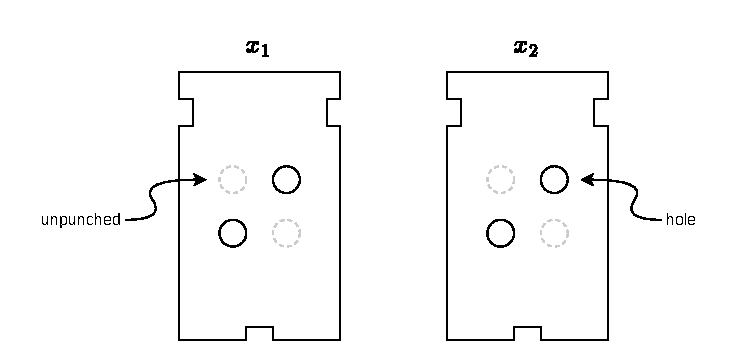
\includegraphics[scale=1.0]{Figures/Problem7.28.pdf} \\
Collection of cards for $\phi = (x_1 \vee x_1 \vee x_2) \wedge (\overline{x_1} \vee \overline{x_2} \vee \overline{x_2})$.
\end{center}

\end{document}